\documentclass[conference]{IEEEtran}
\IEEEoverridecommandlockouts

\usepackage{cite}
\usepackage{amsmath,amssymb}
\usepackage{booktabs}
\usepackage{graphicx}
\usepackage{url}

\begin{document}

\title{A Reproducible Synthetic-Data Pipeline for Telecom Customer Churn Prediction with Explainable Retention Recommendations}

\author{\IEEEauthorblockN{[AUTHOR NAME REQUIRED]}
\IEEEauthorblockA{\textit{[Department and Institution Required]}\\
\textit{[City, Country Required]}\\
[E-mail Required]}}

\maketitle

\begin{abstract}
Customer churn prediction can help a telecommunications provider prioritize retention activity before a customer terminates service. This paper reports the implemented behaviour of a reproducible churn-prediction application comprising a Python machine-learning pipeline, a Flask application programming interface (API), and a React dashboard. Unlike studies based on operator data, the current implementation generates a controlled synthetic panel of 1,000 customers with six monthly observations per customer (6,000 rows). It aggregates the panel to one record per customer, derives service-usage, complaint, recharge, customer-lifetime-value (CLV), and behavioural-change variables, and evaluates Logistic Regression, Random Forest, and XGBoost classifiers. Numeric variables are median-imputed and standardized; categorical variables are most-frequent-imputed and one-hot encoded. In a stratified 80:20 hold-out evaluation with random state 42, Logistic Regression achieved the highest ROC--AUC (0.8329), with accuracy 0.7900, precision 0.7593, recall 0.5857, and F1-score 0.6613. Random Forest achieved slightly higher precision (0.7647), whereas XGBoost achieved the highest recall (0.6143), but neither exceeded the selected model in ROC--AUC. The dashboard exposes individual risk predictions and rule-based retention recommendations using predicted risk and CLV. The results demonstrate an auditable prototype, while its synthetic label-generation mechanism, preprocessing-before-splitting sequence, and lack of a real external validation set limit operational interpretation.
\end{abstract}

\begin{IEEEkeywords}
Telecommunications, customer churn prediction, synthetic data, Logistic Regression, explainable artificial intelligence, SHAP, retention recommendation.
\end{IEEEkeywords}

\section{Introduction}
Customer attrition reduces the recurring-revenue base of subscription businesses and motivates early identification of customers likely to discontinue service. Churn prediction frames this task as supervised binary classification: customer attributes and recent behaviour are used to estimate the probability of a churn event. In an intervention setting, an estimate is useful only when it can be translated into a ranked work list and a defensible action. Prior churn work therefore emphasizes both predictive accuracy and the economic consequences of whom a campaign targets \cite{verbeke}.

The present project was built as an end-to-end demonstration rather than as an analysis of an operator-owned dataset. It intentionally creates monthly customer records containing demographics, contractual attributes, service characteristics, usage, complaints, recharges, and short complaint texts. The churn label is generated in the same program from a transparent probability rule: month-to-month contracts, short tenure, and low average monthly revenue increase the base probability. The code then aggregates each customer's monthly history, fits candidate classifiers, and exposes a prediction service to a browser dashboard.

This design creates a useful educational and engineering artifact, but it also changes the research claim that is appropriate. The objective is not to establish a deployable telecom model or to report superiority over published systems. It is to document a reproducible prototype that compares three implemented classifiers, makes its data-generating assumptions explicit, and connects a selected model to a user interface and retention workflow. The contributions are: 1) a reproducible six-month synthetic customer panel and customer-level feature construction procedure; 2) an implemented comparison of Logistic Regression, Random Forest, and XGBoost under one stratified hold-out protocol; 3) a Flask/React integration that returns churn probabilities, SHAP-based explanations when available, and risk/CLV-based retention suggestions; and 4) a transparent account of limitations that would need correction before evaluation on real telecommunications data.

\section{Related Work}
Churn modelling has long been studied as a customer-relationship-management problem. Neslin \emph{et al.} evaluated the predictive accuracy of churn models using wireless-carrier data and highlighted the importance of modelling choices and target definition \cite{neslin}. Verbeke \emph{et al.} argued that conventional statistical measures alone may not select the most profitable campaign target set, proposing a profit-driven perspective for telecom churn prediction \cite{verbeke}. These studies motivate the project's use of probability estimates and its downstream retention layer, although the current code does not perform profit optimisation.

The classifier choices represent common complementary approaches. Logistic Regression estimates the log-odds of churn as a linear combination of predictors and is readily interpretable. Random Forest aggregates randomized decision trees to reduce variance \cite{breiman}. Gradient-boosted trees build an additive model by sequentially minimizing a loss function \cite{friedman}, while XGBoost provides an efficient regularized tree-boosting implementation \cite{chen}. These techniques are included as separate candidates in the repository; no voting ensemble is implemented.

Churn data can be imbalanced, so high accuracy alone may obscure weak detection of the attrition class. Burez and Van den Poel discuss this problem specifically for customer churn \cite{burez}. Accordingly, this study reports precision, recall, F1-score, and ROC--AUC in addition to accuracy. ROC analysis compares the ranking capability of probability models across thresholds \cite{fawcett}. The project also contains a SHAP explainability module. SHAP assigns feature attributions to a particular prediction and provides a unified framework for additive feature attribution \cite{lundberg}. The gap addressed here is practical rather than algorithmic: a small, reproducible pipeline links synthetic longitudinal records, conventional classifier comparison, explanation code, and a retention-facing interface.

\section{Dataset and Problem Formulation}
\subsection{Synthetic Data Source and Composition}
The only dataset source in the project is \texttt{create\_sample\_data} in \texttt{backend/main.py}; no CSV, database, or external data URL is present. With its main-program arguments, the function uses NumPy seed 42 and creates 1,000 customer identifiers over months 0--5, producing 6,000 monthly rows. The verified run contains 3,906 non-churn monthly rows and 2,094 churn monthly rows. Since the label is constant for all six records of a customer, the customer-level modelling dataset has 651 non-churn customers and 349 churn customers.

At the monthly level, the raw variables are customer identifier, month, age, tenure, average monthly revenue, contract type, internet service, phone service, data usage, complaints, recharges, complaint text, and churn. Contract type takes month-to-month, one-year, or two-year values; internet service takes DSL, fiber optic, or no service. The project defines churn as a generated binary response, not as a documented service-termination event from an operator. Consequently, its numerical results quantify recovery of the program's simulated pattern and must not be interpreted as a real-world churn rate.

\subsection{Prediction Task}
Let each aggregated customer record be represented by a feature vector $\mathbf{x}_i\in\mathbb{R}^{d}$ and its generated label by $y_i\in\{0,1\}$, where 1 denotes churn. A classifier estimates
\begin{equation}
p_i=P(y_i=1\mid\mathbf{x}_i).
\end{equation}
For a threshold $\tau$, the predicted label is $\hat{y}_i=1$ when $p_i\geq\tau$ and 0 otherwise. The training code uses each estimator's default classification threshold for class predictions and uses $p_i$ for ROC--AUC. The selected model is the one that maximizes hold-out ROC--AUC, not accuracy or F1-score.

\section{Proposed Methodology}
\subsection{Feature Construction and Aggregation}
The pipeline orders records by customer identifier and month. It computes a rolling three-month mean and standard deviation of data usage, the one-month difference in usage (\texttt{usage\_trend}), cumulative complaints, complaint change (\texttt{complaints\_increase}), rolling recharge frequency, and recharge change (\texttt{recharge\_trend}). Missing values introduced by rolling calculations are back-filled, forward-filled, and finally replaced with zero. CLV is calculated as
\begin{equation}
\mathrm{CLV}=\mathrm{avg\_monthly\_revenue}\times\mathrm{tenure}.
\end{equation}

The feature engineer attempts sentiment analysis on complaint text using \texttt{nlptown/bert-base-multilingual-uncased-sentiment}. During the verified execution, the transformer model was unavailable and all sentiment scores were set to the implemented neutral fallback, 0.5. Thus, sentiment was not an empirically learned signal in this run.

For modelling, the latest monthly record is merged with per-customer aggregate statistics: mean, standard deviation, minimum, and maximum data usage; total and mean complaints; total and mean recharges; and number of monthly records. The feature-selection list retains 19 predictors: numeric or Boolean-valued predictors plus the categorical fields \texttt{contract\_type} and \texttt{internet\_service}. Together with the label, the customer-level dataframe has 20 columns. Following one-hot encoding, the processed matrix has 22 columns.

\subsection{Preprocessing and Data Splitting}
\texttt{DataPreprocessor} identifies object/category columns as categorical and numerical dtypes as numeric. It applies median imputation and \texttt{StandardScaler} to numeric columns. It applies most-frequent imputation and \texttt{OneHotEncoder(handle\_unknown='ignore', sparse\_output=False)} to categorical columns. The 1,000-by-22 processed matrix is then divided with \texttt{train\_test\_split(test\_size=0.2, random\_state=42, stratify=y)}, yielding 800 training and 200 test customers.

The order matters: the repository fits the preprocessor to the whole customer-level feature matrix before the hold-out split. This permits hold-out covariate information to influence transformations. It is reported as an implementation fact, not endorsed as best practice. A production-quality evaluation should split raw customer records first and fit all learned preprocessing steps only on training data.

\subsection{Models, Selection, and Retention Process}
Table~\ref{tab:models} lists the implemented model configurations. No hyperparameter search, resampling method, threshold optimization, calibration step, or ensemble voting appears in the training code. Each classifier is evaluated using accuracy, positive-class precision, recall, F1-score, and ROC--AUC; the model with maximum ROC--AUC is retained and may be serialized through \texttt{joblib}.

\begin{table}[!t]
\caption{Implemented model configurations}
\label{tab:models}
\centering
\begin{tabular}{ll}
\toprule
Model & Implemented configuration \\
\midrule
Logistic Regression & \texttt{max\_iter=1000} \\
Random Forest & \texttt{n\_estimators=100} \\
XGBoost & \texttt{eval\_metric='logloss'}; defaults otherwise \\
\bottomrule
\end{tabular}
\end{table}

For the selected model, the explainability component returns local SHAP-based feature contributions and may render a global SHAP summary plot. The existing plot ranks \texttt{data\_usage\_mean} visually as the most spread feature contribution, followed by complaint and data-usage aggregate variables. No numerical mean-absolute-SHAP table is emitted by the code.

\texttt{RetentionEngine} assigns High risk for probabilities at least 0.7, Medium for probabilities from 0.4 to less than 0.7, and Low otherwise. It marks CLV at least 1,000 as High value. A risk/value lookup selects a recommendation such as a premium retention package or monitoring. The API also computes an illustrative potential-revenue value as monthly charges multiplied by 24 and multiplies it by risk and an assumed success rate. These are dashboard heuristics, not measured savings or causal treatment effects.

\section{System Architecture and Implementation}
The executable architecture is: synthetic monthly generator $\rightarrow$ feature engineering and customer-level aggregation $\rightarrow$ preprocessing $\rightarrow$ classifier comparison $\rightarrow$ best-by-ROC--AUC model, SHAP explanation, and retention engine $\rightarrow$ Flask REST API $\rightarrow$ React dashboard. The Python requirements name pandas, NumPy, scikit-learn, XGBoost, Transformers, PyTorch, SHAP, Matplotlib, Seaborn, Flask, and Flask-CORS. The web client is implemented with React 19.2 and Vite 7.3.

The API initializes a smaller 100-customer, six-month synthetic dataset when it starts; this API training mode is distinct from the 1,000-customer main-program experiment reported in Section~\ref{sec:results}. Incoming dashboard payloads are mapped into the preprocessor schema, with unavailable fields filled by neutral defaults. The \texttt{/api/predict} endpoint returns a probability and High/Low label at a 0.5 threshold. The \texttt{/api/retention-advice} endpoint applies the risk/CLV heuristics, while \texttt{/api/run-pipeline} starts the API's training flow.

\section{Experimental Results and Analysis}\label{sec:results}
\subsection{Verified Hold-out Results}
Table~\ref{tab:performance} reproduces the output from an execution of the repository's 1,000-customer path under its fixed seed and installed library environment. Logistic Regression is selected because its ROC--AUC is 0.8329, the largest among the three candidates. Its 0.7900 accuracy means 158 of 200 hold-out customers were classified correctly. Its precision of 0.7593 indicates that 75.93\% of positive churn flags were correct, while recall of 0.5857 indicates that 41 of the 70 hold-out churn customers were detected.

\begin{table*}[!t]
\caption{Stratified 80:20 hold-out performance from the verified 1,000-customer synthetic-data run}
\label{tab:performance}
\centering
\begin{tabular}{lccccc}
\toprule
Model & Accuracy & Precision & Recall & F1-score & ROC--AUC \\
\midrule
Logistic Regression & \textbf{0.7900} & 0.7593 & 0.5857 & \textbf{0.6613} & \textbf{0.8329} \\
Random Forest & 0.7850 & \textbf{0.7647} & 0.5571 & 0.6446 & 0.8173 \\
XGBoost & 0.7600 & 0.6719 & \textbf{0.6143} & 0.6418 & 0.7995 \\
\bottomrule
\end{tabular}
\end{table*}

The ROC--AUC result suggests that the linear model ranked churners above non-churners more consistently in this synthetic dataset than the tree-based alternatives. This is plausible because the label generator itself uses a small set of additive rule effects. It is not evidence that Logistic Regression would generally outperform tree models on actual telecom data; tree methods may benefit when real interaction effects and non-linearities are present.

The Logistic Regression confusion matrix is shown in Table~\ref{tab:cm}. With churn as the positive class, it contains 117 true negatives, 13 false positives, 29 false negatives, and 41 true positives. False negatives are consequential when a provider misses a customer who might otherwise receive a retention intervention. Conversely, false positives receive unnecessary outreach. The choice of threshold should be determined from real campaign cost, intervention capacity, and expected retention benefit; the project does not contain this analysis.

\begin{table}[!t]
\caption{Logistic Regression confusion matrix on the 200-customer hold-out set}
\label{tab:cm}
\centering
\begin{tabular}{lcc}
\toprule
Actual / predicted & Non-churn & Churn \\
\midrule
Non-churn & 117 & 13 \\
Churn & 29 & 41 \\
\bottomrule
\end{tabular}
\end{table}

The dataset is moderately imbalanced at the customer level (34.9\% churn). The code stratifies the split, maintaining 130 non-churn and 70 churn customers in the test partition, but it does not resample or use class weights. Thus, F1-score complements accuracy. No confidence intervals, repeated splits, or cross-validation results were produced for this run; reliability beyond this fixed split is information required.

\subsection{Existing and Recommended Visualizations}
Fig.~\ref{fig:shap} uses the existing \texttt{feature\_importance.png} file. It should be retained only after confirming it was generated by the exact reported run. Additional, currently ungenerated artifacts should include a customer-level class-distribution bar chart, hold-out ROC curves, and a confusion-matrix heat map. These would be derived from the same code and data and should not be represented as completed figures before generation.

\begin{figure}[!t]
\centering
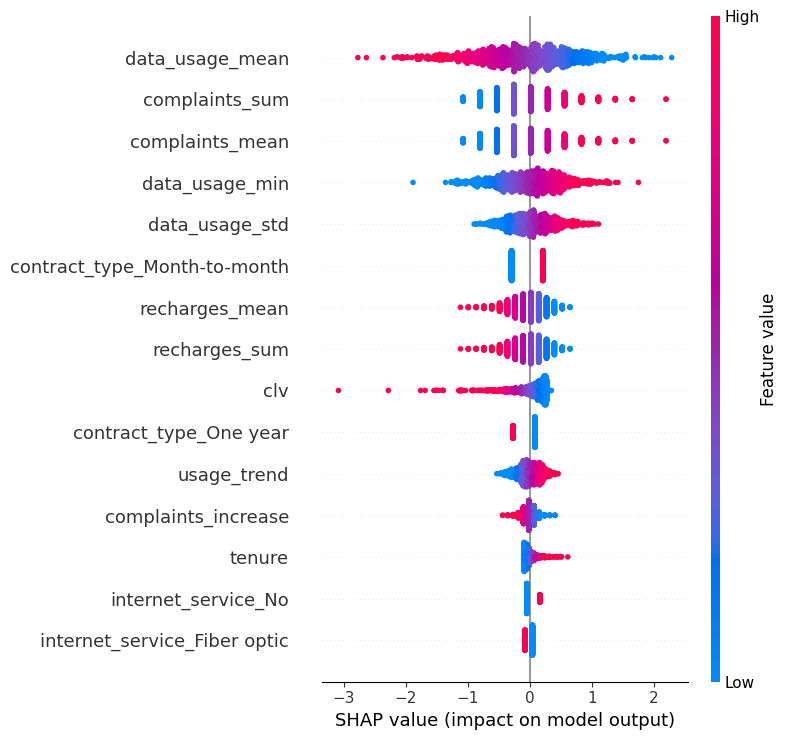
\includegraphics[width=\columnwidth]{feature_importance.png}
\caption{Existing global SHAP summary plot for the selected model.}
\label{fig:shap}
\end{figure}

\section{Discussion}
The project demonstrates how an estimated churn probability can be connected to an operational screen. A telecom analyst could prioritize high-probability customers, inspect the available explanation, and select a retention communication. The dashboard's use of CLV produces a simple prioritization mechanism: high-risk/high-CLV customers receive an intensive retention recommendation, whereas low-risk/low-CLV customers receive no immediate action. This structure is readily understandable for demonstration purposes.

The recommendation mechanism must nevertheless be distinguished from a validated retention policy. The code uses thresholds of 0.7 and 0.4, a CLV threshold of 1,000, a fixed 24-month horizon, and assumed retention success rates of 0.7 or 0.8. None is learned from campaign data. These settings can support interface prototyping but cannot establish expected savings. A deployment study would need observed campaign outcomes, offer costs, contact constraints, and an experimental or causal design to measure incremental retention.

The results show a practical trade-off. XGBoost recovers two additional churners relative to Logistic Regression (43 versus 41) but generates eight additional false positives (21 versus 13), and it has lower ROC--AUC. The correct selection depends on whether missing a churner or contacting a stable customer is costlier. Selecting Logistic Regression by ROC--AUC is consistent with the implemented code, but it is not a universal decision rule.

\section{Limitations}
The principal limitation is synthetic-data circularity. Churn is produced from a known simplified rule involving contract type, tenure, and average monthly revenue, and the model is evaluated on records generated by that same program. The results do not provide external validity, establish causal drivers, or demonstrate performance on an operator's changing population.

Second, preprocessing is fitted before splitting, permitting hold-out covariate information to influence transformations. Third, the feature engineer's attempted sentiment model did not load in the verified environment; the neutral fallback means no sentiment signal was actually extracted. Fourth, a single random split is reported without confidence intervals or temporal validation. Fifth, the API trains a smaller fresh synthetic dataset at start-up rather than loading the checked-in serialized model, so dashboard scores need not equal the main-program scores. Finally, some dashboard inputs do not have corresponding training features and are substituted with default values; this limits the fidelity of individual API predictions.

\section{Conclusion and Future Work}
This paper documents a working full-stack telecom churn prototype that generates a six-month synthetic panel, aggregates customer features, compares three classifiers, and surfaces predictions through a Flask/React interface. In the verified 1,000-customer experiment, Logistic Regression was selected by ROC--AUC (0.8329), with accuracy 0.7900 and F1-score 0.6613. The SHAP module and risk/CLV recommendations make the prototype more inspectable than a prediction-only demonstration.

The next credible step is not to claim higher performance but to replace the synthetic generator with a governed real dataset, define churn and intervention outcomes with the provider, split data temporally before preprocessing, and evaluate using repeated or time-based validation. Future work should fit preprocessing and feature engineering on training data only, calibrate probability thresholds to observed campaign economics, persist one verified pipeline for the API, add ROC and confusion-matrix artifacts, and validate whether explanation-informed offers improve retention. Only after those steps would deployment-scale claims be justified.

\begin{thebibliography}{00}
\bibitem{verbeke} W. Verbeke, K. Dejaeger, D. Martens, J. Hur, and B. Baesens, ``New insights into churn prediction in the telecommunication sector: A profit driven data mining approach,'' \emph{European Journal of Operational Research}, vol. 218, no. 1, pp. 211--229, 2012, doi: 10.1016/j.ejor.2011.09.031.
\bibitem{neslin} S. A. Neslin, S. Gupta, W. Kamakura, J. Lu, and C. H. Mason, ``Defection detection: Measuring and understanding the predictive accuracy of customer churn models,'' \emph{Journal of Marketing Research}, vol. 43, no. 2, pp. 204--211, 2006, doi: 10.1509/jmkr.43.2.204.
\bibitem{breiman} L. Breiman, ``Random forests,'' \emph{Machine Learning}, vol. 45, no. 1, pp. 5--32, 2001, doi: 10.1023/A:1010933404324.
\bibitem{friedman} J. H. Friedman, ``Greedy function approximation: A gradient boosting machine,'' \emph{The Annals of Statistics}, vol. 29, no. 5, pp. 1189--1232, 2001, doi: 10.1214/aos/1013203451.
\bibitem{chen} T. Chen and C. Guestrin, ``XGBoost: A scalable tree boosting system,'' in \emph{Proc. 22nd ACM SIGKDD Int. Conf. Knowledge Discovery and Data Mining}, 2016, pp. 785--794, doi: 10.1145/2939672.2939785.
\bibitem{burez} J. Burez and D. Van den Poel, ``Handling class imbalance in customer churn prediction,'' \emph{Expert Systems with Applications}, vol. 36, no. 3, pp. 4626--4636, 2009, doi: 10.1016/j.eswa.2008.05.027.
\bibitem{fawcett} T. Fawcett, ``An introduction to ROC analysis,'' \emph{Pattern Recognition Letters}, vol. 27, no. 8, pp. 861--874, 2006, doi: 10.1016/j.patrec.2005.10.010.
\bibitem{lundberg} S. M. Lundberg and S.-I. Lee, ``A unified approach to interpreting model predictions,'' in \emph{Advances in Neural Information Processing Systems 30}, 2017, pp. 4765--4774.
\end{thebibliography}

\end{document}
